\subsection{Ecualizador de Fase}


\begin{figure}[hbtp]
\caption{Circuito Ecualizador de Fase}
\centering
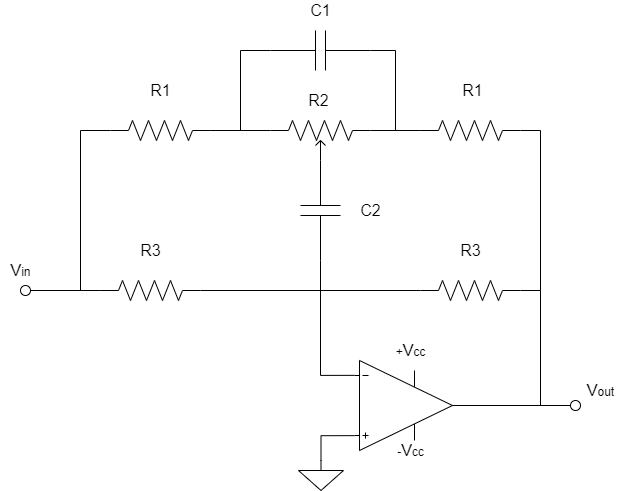
\includegraphics[scale=1]{Informe/Ecualizador de Fase.png}
\end{figure}


\subsection{Análisis matemático}

Para analizar el circuito propuesto, se opto por reemplazar la resistencia variable $R_2$ por dos resistencias las cuales llamaremos $R_{21}$ y $R_{22}$, de esta forma será más fácil poder resolver el circuito propuesto, para esto definimos:


\begin{figure}[H]
	\centering
	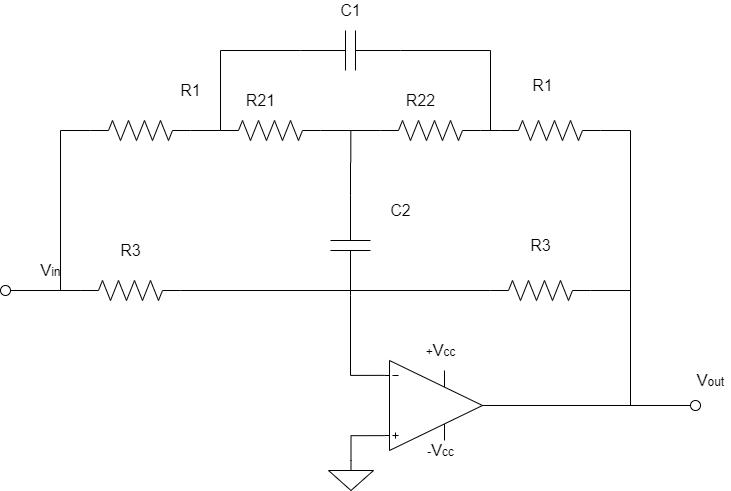
\includegraphics[scale=1]{Informe/EcSinPot.png}
	\caption{Modelo matemático}
\end{figure}
